\begin{frame}{Symmetry Protection of Degenerate Edge}
%\vskip-1.5cm

%\begin{columns}[T]
%    \begin{column}[T]{.5\textwidth}
  $$
    \ket{\psi} = \sum\limits_i \lambda_i \ket{\psi_L^i} \ket{\psi_R^i}
    $$
    \only<1>{
    Inversion symmetriesmap left Schmidt states to  right Schmidt states with the same eigenvalue. Combined with the map that matches each Schmidt state on right to its partner on the left, you get an antiunitary action on sets of degenerate Schmidt states.

    $$
    \mathcal{I} \rightarrow V_{\mathcal{I}}
    $$

    $$
    V_{\mathcal{I}} \ket{e, K} = \ket{-e, K}
    $$
    }

  \only<2>{
    On-site symmetries act unitarily on sets of degenerate Schmidt states.
     $$
     \mathcal{\theta} \rightarrow V_{\mathcal{\theta}}
     $$

    $$
    V_{\mathcal{\theta}} \ket{e, K}  \rightarrow e^{i \theta} \ket{e, K}
    $$

    $$
    V_{\mathcal{\pi}} \ket{e, K} (-1)^{e} \ket{e, K}
    $$
    
    }

  \only<3>{
  Combined inversion and charge parity 

  }


    


 %   \end{column}
  %  \begin{column}[T]{.5\textwidth}
    
   % \end{column}
%\end{columns}
\end{frame}

% \begin{block}{1D Symmetry Protection}
%       \bi
%       \only<1>{
%       \item[] On-site symmetries $g$ come with projective representation $V_g$
%       \item $V_g$ acts on sets of degenerate Schmidt states
%       \item Charge and translation represented linearly on edge
%       }
%       \only<2>{
%       \item[] Time reversal symmetry $\tau$ represented by antiunitary    $V_{\tau} K$ on the edge
%       \item $\tau^2 = +1$ on this edge
%       }
%       \only<3>{
%       \item[] Inversion $\mathcal{I}$
%       \item  $\mathcal{I}$ in combination with swapping Schmidt states represented by antiunitary operation $V_{\mathcal{I}} K$ on the edge
%       \item $\mathcal{I}^2 = V_{\mathcal{I}} V_{\mathcal{I}}^{*} = 1$
      
%       \item[] Inversion $\mathcal{I}$ combined with $\mathcal{\pi} = e^{i\pi N}$
%       \item  $\mathcal{\pi I}$ represented antiunitarily on the edge
%        by $V_{\mathcal{\pi I}} K$
%       \item $(\mathcal{\pi I})^2 = 1$ but $V_{\mathcal{\pi I}} 
%       V_{\mathcal{\pi I}}^{*} = -1$
%       }
%       \ei
%     \end{block}
%     \end{column}
%     \begin{column}[T]{.4\textwidth}
%       \vskip2cm
%       \begin{figure}
%         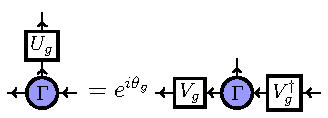
\includegraphics[width=\textwidth]{group_sym.pdf}